\documentclass[12pt]{article}

\usepackage{amsmath, mathtools}
\usepackage{amsfonts}
\usepackage{amssymb}
\usepackage{graphicx}
\usepackage{colortbl}
\usepackage{xr}
\usepackage{hyperref}
\usepackage{longtable}
\usepackage{xfrac}
\usepackage{tabularx}
\usepackage{float}
\usepackage{siunitx}
\usepackage{booktabs}
\usepackage{caption}
\usepackage{pdflscape}
\usepackage{afterpage}
\usepackage{enumerate}
\usepackage[shortlabels]{enumitem}
\usepackage{adjustbox}

\usepackage[round]{natbib}

%\usepackage{refcheck}

\hypersetup{
    bookmarks=true,         % show bookmarks bar?
      colorlinks=true,       % false: boxed links; true: colored links
    linkcolor=red,          % color of internal links (change box color with linkbordercolor)
    citecolor=green,        % color of links to bibliography
    filecolor=magenta,      % color of file links
    urlcolor=cyan           % color of external links
}

%% Comments

\usepackage{color}

\newif\ifcomments\commentstrue %displays comments
%\newif\ifcomments\commentsfalse %so that comments do not display

\ifcomments
\newcommand{\authornote}[3]{\textcolor{#1}{[#3 ---#2]}}
\newcommand{\todo}[1]{\textcolor{red}{[TODO: #1]}}
\else
\newcommand{\authornote}[3]{}
\newcommand{\todo}[1]{}
\fi

\newcommand{\wss}[1]{\authornote{blue}{SS}{#1}} 
\newcommand{\plt}[1]{\authornote{magenta}{TPLT}{#1}} %For explanation of the template
\newcommand{\an}[1]{\authornote{cyan}{Author}{#1}}

%% Common Parts

\newcommand{\progname}{Software Engineering} % PUT YOUR PROGRAM NAME HERE
\newcommand{\authname}{Team 16, Durum Wheat Semolina
	\\ Alexander Moica
	\\ Yasmine Jolly
	\\ Jeffrey Wang
	\\ Jack Theriault
	\\ Catherine Chen
	\\ Justina Srebrnjak } % AUTHOR NAMES                 

\usepackage{hyperref}
    \hypersetup{colorlinks=true, linkcolor=blue, citecolor=blue, filecolor=blue,
                urlcolor=blue, unicode=false}
    \urlstyle{same}
                                


% For easy change of table widths
\newcommand{\colZwidth}{1.0\textwidth}
\newcommand{\colAwidth}{0.13\textwidth}
\newcommand{\colBwidth}{0.82\textwidth}
\newcommand{\colCwidth}{0.1\textwidth}
\newcommand{\colDwidth}{0.05\textwidth}
\newcommand{\colEwidth}{0.8\textwidth}
\newcommand{\colFwidth}{0.17\textwidth}
\newcommand{\colGwidth}{0.5\textwidth}
\newcommand{\colHwidth}{0.28\textwidth}

% Used so that cross-references have a meaningful prefix
\newcounter{defnum} %Definition Number
\newcommand{\dthedefnum}{GD\thedefnum}
\newcommand{\dref}[1]{GD\ref{#1}}
\newcounter{datadefnum} %Datadefinition Number
\newcommand{\ddthedatadefnum}{DD\thedatadefnum}
\newcommand{\ddref}[1]{DD\ref{#1}}
\newcounter{theorynum} %Theory Number
\newcommand{\tthetheorynum}{T\thetheorynum}
\newcommand{\tref}[1]{T\ref{#1}}
\newcounter{tablenum} %Table Number
\newcommand{\tbthetablenum}{T\thetablenum}
\newcommand{\tbref}[1]{TB\ref{#1}}
\newcounter{assumpnum} %Assumption Number
\newcommand{\atheassumpnum}{P\theassumpnum}
\newcommand{\aref}[1]{A\ref{#1}}
\newcounter{goalnum} %Goal Number
\newcommand{\gthegoalnum}{P\thegoalnum}
\newcommand{\gsref}[1]{GS\ref{#1}}
\newcounter{instnum} %Instance Number
\newcommand{\itheinstnum}{IM\theinstnum}
\newcommand{\iref}[1]{IM\ref{#1}}
\newcounter{reqnum} %Requirement Number
\newcommand{\rthereqnum}{P\thereqnum}
\newcommand{\rref}[1]{R\ref{#1}}
\newcounter{nfrnum} %NFR Number
\newcommand{\rthenfrnum}{NFR\thenfrnum}
\newcommand{\nfrref}[1]{NFR\ref{#1}}
\newcounter{lcnum} %Likely change number
\newcommand{\lthelcnum}{LC\thelcnum}
\newcommand{\lcref}[1]{LC\ref{#1}}
\newcounter{ulcnum} %Unlikely change number
\newcommand{\ltheulcnum}{ULC\theulcnum}
\newcommand{\ulcref}[1]{ULC\ref{#1}}
\newcounter{FRCounter}
\setcounter{FRCounter}{1}
\newcommand{\FillFRNumber}{\textbf{FR\arabic{FRCounter}.} \stepcounter{FRCounter}}

\usepackage{fullpage}

\newcommand{\deftheory}[9][Not Applicable]
{
\newpage
\noindent \rule{\textwidth}{0.5mm}

\paragraph{RefName: } \textbf{#2} \phantomsection 
\label{#2}

\paragraph{Label:} #3

\noindent \rule{\textwidth}{0.5mm}

\paragraph{Equation:}

#4

\paragraph{Description:}

#5

\paragraph{Notes:}

#6

\paragraph{Source:}

#7

\paragraph{Ref.\ By:}

#8

\paragraph{Preconditions for \hyperref[#2]{#2}:}
\label{#2_precond}

#9

\paragraph{Derivation for \hyperref[#2]{#2}:}
\label{#2_deriv}

#1

\noindent \rule{\textwidth}{0.5mm}

}

\begin{document}

\title{Software Requirements Specification for \progname} 
\author{Team 16, Durum Wheat Semolina\\Catherine Chen, Yasmine Jolly,\\ Jeffrey Wang, Jack Theriault,\\ Alex 
Moica, Justina Srebrnjak}
\date{\today}
	
\maketitle

~\newpage

\pagenumbering{roman}

\tableofcontents

~\newpage

\section*{Revision History}

\begin{tabularx}{\textwidth}{p{3cm}p{2cm}X}
\toprule {\bf Date} & {\bf Version} & {\bf Notes}\\
\midrule
October 19, 2022 & 1.0 & Initial Version\\
November 1, 2022 & 1.1 & Migrated Additional Requirements from Hazard Analysis\\
March 14, 2023 & 1.2 & Updated NFR/FR with testing considerations\\
March 31, 2023 & 2.0 & Updated with profile and BMI elements, Removed some NFRs\\
\bottomrule
\end{tabularx}

~\newpage

\pagenumbering{arabic}

\plt{This SRS template is based on \citet{SmithAndLai2005, SmithEtAl2007}.  It
  will get you started.  You should not modify the section headings, without
  first discussing the change with the course instructor.  Modification means
  you are not following the template, which loses some of the advantage of a
  template, especially standardization.  Although the bits shown below do not
  include type information, you may need to add this information for your
  problem.  If you are unsure, please can ask the instructor.}

\plt{Feel free to change the appearance of the report by modifying the LaTeX
  commands.}

\plt{This template document assumes that a single program is being documented.
  If you are documenting a family of models, you should start with a commonality
  analysis.  A separate template is provided for this.  For program
  families you should look at \cite{Smith2006, SmithMcCutchanAndCarette2017}.
  Single family member programs are often programs based on a single physical
  model.  General purpose tools are usually documented as a family.  Families of
  physical models also come up.}

\plt{The SRS is not generally written, or read, sequentially.  The SRS is a
  reference document.  It is generally read in an ad hoc order, as the need
  arises.  For writing an SRS, and for reading one for the first time, the
  suggested order of sections is:
\begin{itemize}
\item Goal Statement
\item Instance Models
\item Requirements
\item Introduction
\item Specific System Description
\end{itemize}
}

\plt{Guiding principles for the SRS document:
\begin{itemize}
\item Do not repeat the same information at the same abstraction level.  If
  information is repeated, the repetition should be at a different abstraction
  level.  For instance, there will be overlap between the scope section and the
  assumptions, but the scope section will not go into as much detail as the
  assumptions section.
\end{itemize}
}

\plt{The template description comments should be disabled before submitting this
  document for grading.}

\plt{You can borrow any wording from the text given in the template.  It is part
  of the template, and not considered an instance of academic integrity.  Of
  course, you need to cite the source of the template.}

\plt{When the documentation is done, it should be possible to trace back to the
  source of every piece of information.  Some information will come from
  external sources, like terminology.  Other information will be derived, like
  General Definitions.}

\plt{An SRS document should have the following qualities: unambiguous,
  consistent, complete, validatable, abstract and traceable.}

\plt{The overall goal of the SRS is that someone that meets the Characteristics
  of the Intended Reader (Section~\ref{sec_IntendedReader}) can learn,
  understand and verify the captured domain knowledge.  They should not have to
  trust the authors of the SRS on any statements.  They should be able to
  independently verify/derive every statement made.}

\section{Introduction}

\plt{The introduction section is written to introduce the problem.  It starts
  general and focuses on the problem domain. The general advice is to start with
a paragraph or two that describes the problem, followed by a ``roadmap''
paragraph.  A roadmap orients the reader by telling them what sub-sections to
expect in the Introduction section.}

\subsection{Purpose of Document}

This document describes the requirements for 'Utrition'. It will provide a 
detailed overview of the application, and a comprehensive description of the 
software's functional and non-functional requirements, as well as other details 
relevant to the product. The template for this document is a modified version 
of the Volere template \citep{RobertsonAndRobertson2012}.


\plt{This section summarizes the purpose of the SRS document.  It does not focus
  on the problem itself.  The problem is described in the ``Problem
  Description'' section (Section~\ref{Sec_pd}).  The purpose is for the document
  in the context of the project itself, not in the context of this course.
  Although the ``purpose'' of the document is to get a grade, you should not
  mention this.  Instead, ``fake it'' as if this is a real project.  The purpose
  section will be similar between projects.  The purpose of the document is the
  purpose of the SRS, including communication, planning for the design stage,
  etc.}

\subsection{Scope of Requirements} 
When considering the files the user uploads to the system, the requirements of 
this document are constrained to consider only a subset of all possible file 
types. Furthermore, requirements are created under the impression that files 
are of a manageable size, and are of food objects identifiable by a machine 
learning model. Lastly, we assume the user possesses sufficient knowledge to 
access the system, and does so with internet through a machine capable of 
running most modern applications. That is to say, the user possesses sufficient 
hardware capabilities to access all capabilities of the system.

\plt{Modelling the real world requires simplification.  The full complexity of
  the actual physics, chemistry, biology is too much for existing models, and
  for existing computational solution techniques.  Rather than say what is in
  the scope, it is usually easier to say what is not.  You can think of it as
  the scope is initially everything, and then it is constrained to create the
  actual scope.  For instance, the problem can be restricted to 2 dimensions, or
  it can ignore the effect of temperature (or pressure) on the material
  properties, etc.}  

\plt{The scope section is related to the assumptions section
  (Section~\ref{sec_assumpt}).  However, the scope and the assumptions are not
  at the same level of abstraction.  The scope is at a high level.  The focus is
  on the ``big picture'' assumptions.  The assumptions section lists, and
  describes, all of the assumptions.}

\subsection{Characteristics of Intended Reader} \label{sec_IntendedReader}
This document is intended for the developers and testers working on this 
system, so that the requirements of the system can be communicated throughout 
the development process. Readers should have an understanding of the software 
design life cycle as well as the ability to read discrete math at a 
university-level in order to fully understand the contents and 
equations used in this document.

\plt{This section summarizes the skills and knowledge of the readers of the
  SRS.  It does NOT have the same purpose as the ``User Characteristics''
  section (Section~\ref{SecUserCharacteristics}).  The intended readers are the
  people that will read, review and maintain the SRS.  They are the people that
  will conceivably design the software that is intended to meet the
  requirements.  The user, on the other hand, is the person that uses the
  software that is built.  They may never read this SRS document.  Of course,
  the same person could be a ``user'' and an ``intended reader.''}

\plt{The intended reader characteristics should be written as unambiguously and
  as specifically as possible.  Rather than say, the user should have an
  understanding of physics, say what kind of physics and at what level.  For
  instance, is high school physics adequate, or should the reader have had a
  graduate course on advanced quantum mechanics?}

\subsection{Organization of Document}

The rest of the SRS will discuss the purpose and context of the system, 
followed by the functional requirements it must satisfy. Then the document will 
mention its non-functional requirements, providing justifications for each. 
This is followed by a discussion of potential issues that may arise during the 
project's development. Lastly, the document lists likely and unlikely 
changes, and includes a traceability matrix for the system.

\plt{This section provides a roadmap of the SRS document.  It will help the
  reader orient themselves.  It will provide direction that will help them
  select which sections they want to read, and in what order.  This section will
  be similar between project.}

\section{Project Drivers }

\subsection{The Purpose of the Project}

The purpose of the Utrition application is to help individuals learn more about maintaining a healthy lifestyle and assisting them in making wise decisions. This application is built for the users to learn more about what their meals consist of by breaking down the calories and nutrition facts of the food they intend on eating or purchasing.  

\subsection{The Stakeholders }

\subsubsection{The Client}  

The client requesting this application is the instructor of the Software Engineering 4G06, Dr. Smith and the teaching assistants. This application is expected to be unique as compared to products in the market that attempt to tackle a similar problem as per the client's request.  

\subsubsection{The Customers} 

The customers of Utrition are assumed to be health-conscious individuals that are attempting to improve their daily eating habits by tracking the nutrients and calories found in their previous meals. 

\subsubsection{Other Stakeholders}
Other stakeholders of the Utrition application consist of grocery stores, restaurants, and gyms. These stakeholders are affected as the users of this program may change their previous dynamic with these stakeholders due to their increase in knowledge of the nutrients they are consuming. In terms of a grocery store, their stock may be affected due to an increase in individuals buying more health-conscious foods. For restaurants, they might experience a decrease in customers if users develop a preference to cook from home in order to eat healthier. Lastly, gyms might see an increase in attendees if Utrition users wish to burn off extra calories they discover they have consumed.

\subsection{Mandated Constraints} 

As we wish to make Utrition as accurate as possible when identifying food, the application will only be trained for individual food items or ingredients rather than whole meals. For example, the user is expected to provide a picture of lettuce rather than an entire sandwich if they wish to track that lettuce appeared in their sandwich. This constraint is to ensure that the user gets an accurate estimate of exactly the nutritional value of their meal since the application may not detect all separate food items in one picture. 

\subsection{Naming Conventions and Terminology}
\renewcommand{\arraystretch}{1.2}
\begin{tabular}{l l} 
	\toprule		
	\textbf{symbol} & \textbf{description}\\
	\midrule 
	A & Assumption\\
	API & Application Programming Interface\\
	App & Application\\
	CP & Cultural and Political Requirement\\
	FR & Functional Requirement\\
	LC & Likely Change\\
	LF & Look and Feel Requirement\\
	LR & Legal Requirement\\
	MS & Maintainability and Support Requirement\\
	OE & Operational and Environmental Requirement\\
	PR & Performance Requirement\\
	SR & Security Requirement\\
	SRS & Software Requirements Specification\\
	UH & Usability and Humanity Requirement\\
	UI & User Interface\\
	ULC & Unlikely Change\\
	Standard image types & These are image files of extensions which include .png, .jpg, .jpeg. \\
\end{tabular}\\

\subsection{Relevant Facts and Assumptions } 

\begin{itemize}
	
	\item [A1:] The user has an understanding of how to effectively utilize web based applications.
	
	\item [A2:] The user is able to upload a food image to Utrition. This can be a saved image or a new image taken using a device.
	
	\item [A3:] There is an assumption that the client will only take a picture of individual ingredients. 

	\item [A4:] The user is expected to have knowledge of the metric system as Utrition will be outputting nutritional value data in grams and calories.
	
	\item [A5.] The user is expected to have internet access while using Utrition.

\end{itemize}

\section{Functional Requirements}

\subsection{The Scope of the Work and the Product}

The scope of the project is to develop a nutrition tracking application to identify food items based on an image and derive nutritional data from the classified food. This application can be installed on the user's system and will have comprehensive software documentation.

\subsubsection{The Context of the Work}
\begin{figure}[H]
	\centering
	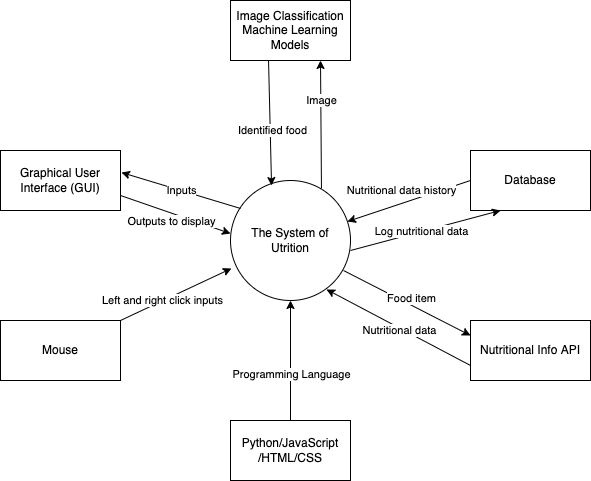
\includegraphics[scale=0.6]{work_context_diagram.png}
	\caption{Work Context Diagram}
\end{figure}


\subsubsection{Work Partitioning}

\begin{tabular}{ |p{5cm}|p{4cm}|p{6.5cm}| }
\hline
\textbf{Event Name}                   & \textbf{Input/Output}                                            & \textbf{Summary}                                                                                                                            \\ 
\hline
System receives image                 & User uploaded image (in) / Pre-processed image (out)             & User uploads an image and it is pre-processed into a format that can be sent to the computer vision algorithm.                              \\ 
\hline
Food identified in image              & Pre-processed image~(in) / Identified food (out)                 & The pre-processed image is processed to identify the food it represents through the use of our machine learning computer vision algorithm.  \\ 
\hline
Nutritional data retrieved            & Identified food(in) / Nutritional data (out)                     & The identified food is passed into a matching algorithm to retrieve the associated nutritional data from all stored nutritional data.       \\ 
\hline
Nutritional data displayed            & Nutritional data (in) / Visual display of nutritional data (out) & The raw nutritional data is transformed into a human readable format and displayed to the user.                                             \\ 
\hline
Nutritional data~logged               & Nutritional data (in) / Logging of data (out)                    & The nutritional data and search information of a user's search is internally logged and persists after the program has exited.              \\ 
\hline
Past nutritional data retrieved       & User mouse input (in) / Nutritional data (out)                   & The user is able to retrieve the nutritional data and search information of their past image uploads.                                       \\ 
\hline
Past nutritional data chart displayed & Nutritional data (in) / Chart (out)                              & Past nutritional data is displayed in a graph, showing past searches and nutritional data through various periods of time.                  \\
\hline
Profile settings logged & Profile data (in) / Saving of data (out)                              & The user inputted profile data is internally saved and persists after the prrogram has exited.                  \\
\hline
BMI related data displayed & Profile data (in) / BMI data (out)                              & The profile data is used to calculate a BMI analysis to be displayed to the user.                  \\
\hline
\end{tabular}

\subsubsection{Individual Product Use Cases}
\begin{figure}[H]
	\centering
	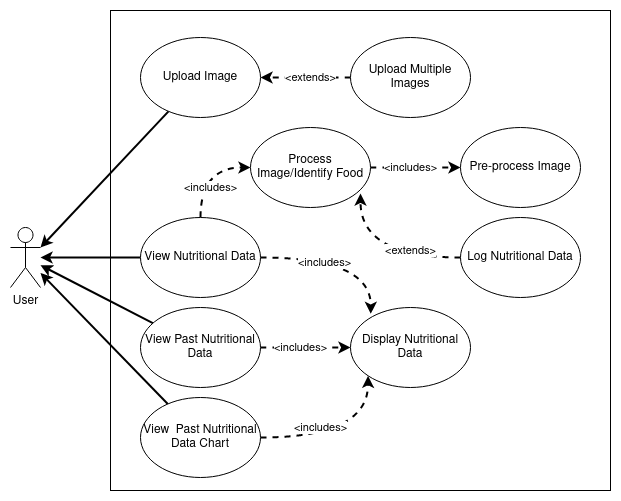
\includegraphics[scale=0.7]{use_case_diagram.png}
	\caption{Use Case Diagram}
\end{figure}

\subsection{Functional Requirements}


\begin{itemize}
    \item [\FillFRNumber] The user must have the ability to upload a digital image of a \textbf{standard image type} to the system.\newline 
    \textbf{Formalization}: $x \in A \mid x = \text{Images}, A = \{\text{\textbf{standard image types}}\}$\newline
    \textbf{Rationale}: In order for the system to identify the food a user is eating, the user would have to upload an image of their food to the system. The image shall be saved on the user’s device, which can then be selected. This will allow for the user to have a simple process of uploading an image, instead of manually inputting the details of what they ate.\newline
    \textbf{Priority}: High
\end{itemize}

\begin{itemize}
    \item [\FillFRNumber] The system will be able to identify the type of food that is captured in an image.\newline 
    \textbf{Formalization}: $\forall x \cdot \exists y \cdot y \in B \mid x = \text{Images}, B = \{\text{food label type}\}$\newline
    \textbf{Rationale}: In order for the system to return the nutritional content of a food, the system must first identify the food present in an image.This will further support the user to have a streamlined experience when uploading an image of the food they ate. \newline
    \textbf{Priority}: High
\end{itemize}

\begin{itemize}
    \item [\FillFRNumber] The system will be able to make an API call to an external database of nutrition facts for a variety of foods, including their macro-nutrients, micro-nutrients, and caloric details.\newline
    \textbf{Rationale}: In order to provide a user with the nutritional regarding their meal, the system must first be able to fetch the nutritional data for a large variety of foods for later use.\newline
    \textbf{Priority}: High
\end{itemize}

\begin{itemize}
    \item [\FillFRNumber] The system will be able to retrieve the nutrition facts for a specific food.\newline
    \textbf{Formalization}: $\forall y \cdot \exists z \cdot z \in C \mid y = \text{food label}, C = \{\text{nutritional data}\}$\newline
    \textbf{Rationale}: In order to provide the user with the nutritional data regarding their meal, the system would have to be able to retrieve the nutritional data for a given food.\newline
    \textbf{Priority}: High
\end{itemize}

\begin{itemize}
	\item [\FillFRNumber] The system will log the nutritional data of a food.\newline
	\textbf{Formalization}: $\forall v \cdot \exists z \cdot z \in C \mid v = \text{logged food label}, C = \{\text{nutritional data}\}$\newline
	\textbf{Rationale}: Nutritional data of a food will be saved for future reference. This system shall be able to fetch previously recorded data for other processes, such as displaying visuals and calculating nutritional summaries. This will support the user to be able to see their history and nutritional trends. \newline 
	\textbf{Priority}: Medium
\end{itemize}

\begin{itemize}
	\item [\FillFRNumber] The user will be able to access the nutritional data of previously logged foods. \newline
	\textbf{Rationale:} Nutritional data found in the database shall be available to be referenced and displayed to the user. This will allow the user to view nutritional details of the food that was previously tracked within the application. \newline
	\textbf{Priority:} Medium
\end{itemize}

\begin{itemize}
	\item [\FillFRNumber] The system will display the nutritional information of a food to the user. \newline
	\textbf{Rationale:} Nutritional data of a particular food item shall be displayed on the user interface, so the user can view the detailed nutritional breakdown of the food.\newline
	\textbf{Priority:} High
\end{itemize}

\begin{itemize}
	\item [\FillFRNumber] The user must have the ability to upload the text of a food as an input to the system.\newline 
	\textbf{Rationale:} Users must have the ability to log the nutritional data of a food through typing the food items they ate. This gives users more upload options for their convenience.\newline
	\textbf{Priority:} High
\end{itemize}

\begin{itemize}
	\item [\FillFRNumber] The user must have the ability to upload multiple texts of food inputs to the system.\newline 
	\textbf{Rationale:} Users must have the ability to log the nutritional data of multiple foods through typing the name of the foods.This allows for a smooth user experience, where multiple foods the user would like to log can be added all at once.\newline
	\textbf{Priority:} High
\end{itemize}

\begin{itemize}
	\item [\FillFRNumber] The user must have the ability to upload a food input by speaking to the system.\newline 
	\textbf{Rationale:} Users must be able to vocally input the food they want the nutritional data for. The user will have another method to upload food for their convenience.\newline
	\textbf{Priority:} Medium
\end{itemize}

\begin{itemize}
	\item [\FillFRNumber] The user must have the ability to upload multiple food inputs by speaking to the system.\newline 
	\textbf{Rationale:} Users must be able to vocally input the foods they want the nutritional data for. This allows users to speak in full, compound sentences as a method of inputting food items to the system. \newline
	\textbf{Priority:} Medium
\end{itemize}

\begin{itemize}
	\item [\FillFRNumber] The system will be able to convert vocal input into text.\newline 
	\textbf{Rationale:} The system must be able to convert voice to text to allow retrieving nutritional data for the input.\newline
	\textbf{Priority:} Medium
\end{itemize}

\begin{itemize}
	\item [\FillFRNumber] The user must have the ability to clear their voice upload from the system. \newline
	\textbf{Rationale:} The system must allow the user to correct their misinputs for the voice input functionality. This will help take pressure off the user to speak perfectly. \newline
	\textbf{Priority:} Medium
\end{itemize}

\begin{itemize}
	\item [\FillFRNumber] The system will be able to identify the type of food(s) that is captured in a complex sentence. \newline
	\textbf{Rationale:} The system must be able to process natural language. This means the system must be able to decipher the food items in a long-winded sentence. Users should be allowed to use their normal speech or texting abilities to input food items. \newline
	\textbf{Priority:} Medium
\end{itemize}

\begin{itemize}
	\item [\FillFRNumber] The user must have the ability to select between uploading food(s) through image, text, or voice. \newline
	\textbf{Rationale:} The system must allow the user to select what type of input they would like to use. This allows the user to have flexibility for input methods according to their needs. \newline
	\textbf{Priority:} High
\end{itemize}

\begin{itemize}
	\item [\FillFRNumber] The system will display the user's most logged food. \newline
	\textbf{Rationale:} Certain users will be interested in what foods they have eaten the most. \newline
	\textbf{Priority:} Low
\end{itemize}

\begin{itemize}
	\item [\FillFRNumber] The system will display the user's total calories consumed for the day. \newline
	\textbf{Rationale:} Users will want to count their calories to ensure they don't go over their daily limit. This will encourage users to be mindful about their consumed foods.\newline
	\textbf{Priority:} Medium
\end{itemize}

\begin{itemize}
	\item [\FillFRNumber] The system will display a summary of the foods consumed and their total calories for each of the past 7 days. \newline
	\textbf{Rationale:} Users will be able to have a more holistic overview of their nutritional state by viewing the breakdown of foods eaten over the week, along with their calories. \newline
	\textbf{Priority:} Medium
\end{itemize}

\begin{itemize}
	\item [\FillFRNumber] The user will be able to access the summary of the foods consumed and their total calories for all days with a food inputted. \newline
	\textbf{Rationale:}  Users will want to access and view their calories and foods they've eaten. \newline
	\textbf{Priority:} Medium
\end{itemize}

\begin{itemize}
	\item [\FillFRNumber] The user will be able to access the Home page, the Upload page, and the Profile page on every page. \newline
	\textbf{Rationale:}  Users will be able to access every page, so their use of Utrition is not restricted. \newline
	\textbf{Priority:} High
\end{itemize}

\begin{itemize}
	\item [\FillFRNumber] The user will be able to delete a previously logged food. \newline
	\textbf{Rationale:}  In the profile page displaying the past foods, the user shall have the flexibility to delete a food that was previously logged. \newline
	\textbf{Priority:} High
\end{itemize}

\begin{itemize}
	\item [\FillFRNumber] The user will be able to input profile statistics related to their health and measurements. \newline
	\textbf{Rationale:}  The user shall have the option to input data related to their health, which will allow for customized BMI related calculations and displays. \newline
	\textbf{Priority:} High
\end{itemize}

\begin{itemize}
	\item [\FillFRNumber] The system shall log the user profile data.\newline
	\textbf{Rationale:}  User profile data will be saved for future reference, and to be used for BMI related functionalities. \newline
	\textbf{Priority:} High
\end{itemize}

\begin{itemize}
	\item [\FillFRNumber] The user will be able to modify the profile statistics.\newline
	\textbf{Rationale:}  Users will have the ability to change their profile statistics in case of the event of a mistake or a change in measurements. \newline
	\textbf{Priority:} Medium
\end{itemize}

\begin{itemize}
	\item [\FillFRNumber] The system shall be able to perform BMI related calculations. \newline
	\textbf{Rationale:}  User profile data will be used for BMI related functionalities, including BMI classification, and the calculation of the recommeded amount of calories to maintain a healthy weight. \newline
	\textbf{Priority:} High
\end{itemize}

\begin{itemize}
	\item [\FillFRNumber] The system shall be able to display BMI related conclusions based on the user profile data. \newline
	\textbf{Rationale:} Users will be able to view their BMI classification, and recommended amount of calories. The system will provide the users with more personal and catered data analysis through the BMI calculations. \newline
	\textbf{Priority:} High
\end{itemize}

\begin{itemize}
	\item [\FillFRNumber] The system shall be able to display a graph of user caloric trends. \newline
	\textbf{Rationale:} Users will be able to see a graphical representation of the calories consumed over time, for another way to visualize their nutritional habits. This can help them reach and stay on track with their nutritional goals. \newline
	\textbf{Priority:} Medium
\end{itemize}

\begin{itemize}
	\item [\FillFRNumber] The system shall be verify the user's request to delete a logged food item.  \newline
	\textbf{Rationale:} In case the user accidentally chooses to delete a logged food item, the system will verify the user's request to ensure it was not done by accident. This prevents unwanted deletions. \newline
	\textbf{Priority:} High
\end{itemize}


\section{Non-Functional Requirements}

\subsection{Look and Feel Requirements}

\subsubsection{Appearance Requirements}

\begin{enumerate}[{LF}1. ]
	\item Utrition’s user interface will be clutter-free.\\
	\textbf{Rationale:} Users must be able to access and read all parts of the user interface. \\
	\textbf{Fit Criteria:} The distance between user interface components must exceed 20 pixels.
\end{enumerate}

\subsubsection{Style Requirements}
\hspace{1.5cm}N/A

\subsection{Usability and Humanity Requirements}

\subsubsection{Ease of Use Requirements}

\begin{enumerate}[{UH}1. ]
	\item The user interface will be easy to navigate. \\
	\textbf{Rationale:} This allows the user to efficiently learn and use Utrition.\\
	\textbf{Fit Criteria:} The user will be able to navigate to the main menu from any page in 2 clicks.
\end{enumerate}

\subsubsection{Personalization and Internationalization Requirements}

\begin{enumerate}[{UH}2. ] 
	\item Utrition will retain the user’s diet history.\\
	\textbf{Rationale:} Users will be able to view their dietary habits and can make nutritional adjustments based on their observations.\\
	\textbf{Fit Criteria:} The user must be able to view every past inputted food item.
	
\end{enumerate}

\subsubsection{Learning Requirements}

\begin{enumerate}[{UH}3. ] 
	\item Utrition will be able to be used by people aged 14 and higher who have received no training on the product.\\
	\textbf{Rationale:} Utrition should be able to be used by all individuals who are concerned with their dietary habits.\\
	\textbf{Fit Criteria:} 90\% of a test panel of the target demographic should be able to upload their food and retrieve the corresponding nutritional facts in under 2 minutes.
\end{enumerate}

\subsubsection{Understandability and Politeness Requirements}

\begin{enumerate}[start=4,label={UH\arabic*.}]
	\item Key information will be easy to understand on Utrition.\\
	\textbf{Rationale:} Users will be more likely to use the web application if they are able to understand it efficiently.\\
	\textbf{Fit Criteria:} Every clickable object will have a symbol associated with it. Calories, fat, sodium, carbohydrates, sugar, and protein will have a symbol associated next to it.
	\item Utrition will not overwhelm the user with information.\\
	\textbf{Rationale:} The user is only concerned with the nutritional information and not the calculations leading up to it.\\
	\textbf{Fit Criteria:} All backend calculations, such as identifying the uploaded food and retrieving the nutritional information, will not be displayed to the user.
\end{enumerate}

\subsubsection{Accessibility Requirements}

\begin{enumerate}[{UH}6. ] 
	\item Utrition will be able to be used by deaf people.\\
	\textbf{Rationale:} Durum Wheat Semolina aims to allow as many individuals as possible to use Utrition.\\
	\textbf{Fit Criteria:} There will be no sound used by the Utrition web application. 
\end{enumerate}

\subsection{Performance Requirements}

\subsubsection{Speed and Latency Requirements}

\begin{enumerate}[start=1,label={PR\arabic*.}]
	\item Switching between different user interface screens will be quick.\\
	\textbf{Rationale:} The user should not have to wait to access different parts of the Utrition web application.\\
	\textbf{Fit Criteria:} The time between the user’s click and displaying the new UI will not exceed 2 seconds.
\end{enumerate}

\subsubsection{Safety-Critical Requirements}
\hspace{1.5cm}N/A

\subsubsection{Precision or Accuracy Requirements}

\begin{enumerate}[start=2,label={PR\arabic*.}]
	\item Identifying and displaying each food item will be done correctly. \\
	\textbf{Rationale:} The web app should provide the user with accurate information. \\
	\textbf{Fit Criteria:} In a test with multiple images, Utrition will identify and display the correct food with an average accuracy of 70\%.
	\item  The displayed nutritional facts will be correct. \\
	\textbf{Rationale:} The nutritional information given to the user should be accurate. \\
	\textbf{Fit Criteria:} In a test with multiple images, Utrition will display the correct nutritional information for an identified food 90\% of the time.
\end{enumerate}

\subsubsection{Reliability and Availibility Requirements}
\hspace{1.5cm}N/A

\subsubsection{Robustness or Fault-Tolerance Requirements}
\hspace{1.5cm}N/A

\subsubsection{Capacity Requirements}

\hspace{1.5cm}N/A


\subsubsection{Scalability or Extensibility Requirements}

\begin{enumerate}[{PR}4. ] 
	\item Utrition will have no limit to the size of the user base for its lifespan. \\
	\textbf{Rationale:} Utrition should be available to all individuals who are health conscious.\\
	\textbf{Fit Criteria:} Utrition is a local web app and does not depend on a server.
\end{enumerate}

\subsubsection{Longevity Requirements}

\begin{enumerate}[{PR}5. ] 
	\item Utrition should operate indefinitely once fully developed.\\
	\textbf{Rationale:} Nutritional food values will never change and people will always want ways to regulate their diet. \\
	\textbf{Fit Criteria:} Utrition will be available to use on GitHub for an indefinite amount of time.
\end{enumerate}

\subsection{Operational and Environmental Requirements}

\subsubsection{Expected Physical Environment}
\hspace{1.5cm}N/A

\subsubsection{Requirements for Interfacing with Adjacent systems}
\hspace{1.5cm}N/A 

\subsubsection{Productization Requirements}
\begin{enumerate}[start=1,label={OE\arabic*.}]
	\item Utrition will be available on GitHub as a public repository.\\
	\textbf{Rationale:} Utrition is free to be used by anyone.\\
	\textbf{Fit Criteria:} Users will be able to find and pull the repository on to their personal device.
	\item Utrition will be able to be installed by any individual aged 14 or older after reading the installation guide on the Utrition GitHub page.\\
	\textbf{Rationale:} Utrition should have a simple installation process. \\
	\textbf{Fit Criteria:} 95\% of a test panel with the intended demographic will be able to install Utrition after reading the installation guide.
\end{enumerate}

\subsubsection{Release Requirements}

\begin{enumerate}[{OE}3. ] 
	\item Utrition will not have any updates after final implementation is complete.\\
	\textbf{Rationale:} Food components and their nutritional value do not change over time which means no updates are needed to keep the system functioning and relevant.\\	
	\textbf{Fit Criteria:} Utrition’s GitHub repository will receive no updates after final implementation.
\end{enumerate}

\subsection{Maintainability and Support Requirements}

\subsubsection{Maintenance Requirements}
\begin{enumerate}[{MS}1. ] 
	\item During development, new data can be used to improve Utrition’s machine learning model.\\
	\textbf{Rationale:} Utrition’s machine learning model can receive new data to improve itself and detect food at 70\% accuracy.\\	
	\textbf{Fit Criteria:} Any backend developer is able to successfully upload new data to Utrition’s machine learning model at any time during development. 
\end{enumerate}

\subsubsection{Supportability Requirements}
\begin{enumerate}[{MS}2. ] 
	\item Technical support related to installation and the use of Utrition will be found in Utrition’s GitHub repository. \\
	\textbf{Rationale:} Users who are not technologically advanced should be able to use Utrition given an installation guide and user manual.\\	
	\textbf{Fit Criteria:} All users will be able to view the support manuals on how to install and use Utrition.
\end{enumerate}

\subsubsection{Adaptability Requirements}
\begin{enumerate}[{MS}3. ] 
	\item Utrition will be used on any computer with access to ".png", ".jpg", or ".jpeg" photo format.\\
	\textbf{Rationale:} The user must be able to upload image files to Utrition in one of these formats. \\
	\textbf{Fit Criteria:} 100\% of the tested Windows, macOS, and Linux devices should be able to use all functionality provided for Utrition.
\end{enumerate}


\subsection{Security Requirements}

\subsubsection{Access Requirements}
\begin{enumerate}[{SR}1. ] 
	\item The entirety of Utrition can be accessed by all individuals. \\
	\textbf{Rationale:} The user has the flexibility to improve Utrition and the right to know what they’re downloading onto their computer.  \\	
	\textbf{Fit Criteria:} Anyone will be able to pull the open-source project from GitHub
\end{enumerate}

\subsubsection{Integrity Requirements}
\begin{enumerate}[{SR}2. ] 
	\item Utrition will periodically save user’s data during use. \\
\textbf{Rationale:} In the event of unexpected shutdown, the user should 
not lose all information from the last session. Periodically saving user 
information will allow users to continue from their last step in the event 
of an unexpected shutdown. \\	
	\textbf{Fit Criteria:} Utrition will save user data ever 3 minutes throughout the 
	application runtime.
\end{enumerate}

\subsubsection{Privacy Requirements}
\begin{enumerate}[{SR}3. ] 
	\item Utrition will store the user’s data locally.\\
	\textbf{Rationale:} Only the user should have to view their stored dietary habits. \\	
	\textbf{Fit Criteria:} Utrition will not contain personalized data from one user on another user's system.
\end{enumerate}

\subsubsection{Audit Requirements}
\hspace{1.5cm}N/A 

\subsubsection{Immunity Requirements}
\hspace{1.5cm}N/A 

\subsection{Cultural or Political Requirements}

\subsubsection{Cultural Requirements}

\begin{enumerate}[{CP}1. ] 
	\item Utrition will not display any culturally insensitive content. \\
	\textbf{Rationale:} Utrition should not show culturally insensitive content since the application is intended for individuals of any race or religion.\\	
	\textbf{Fit Criteria:} 95\% of the test panel agrees that Utrition does not provide any culturally insensitive content to the user.
\end{enumerate}

\subsubsection{Political Requirements}
\hspace{1.5cm}N/A

\subsection{Legal Requirements}
\subsubsection{Compliance Requirements}
\begin{enumerate}[{LR}1. ]
	\item Utrition follows Canada’s Anti-Spam Legislation Requirements for Installing Computer Programs \citep{CanadianInstall}.\\
	\textbf{Rationale:} Durum Wheat Semolina complies with the law to provide an application void of spam and computer viruses.\\
	\textbf{Fit Criteria:} No malicious software will be present in Utrition’s GitHub repository.
\end{enumerate}
\subsubsection{Standards Requirements}
\begin{enumerate}[start=2,label={LR\arabic*.}]
	\item Durum Wheat Semolina follows Canada's "Guide for Publishing Open Source 
	Code" \citep{CanadianCode}.\\
	\textbf{Rationale:} This guide will assist Durum Wheat Semolina in setting up the development environment for Utrition.\\
	\textbf{Fit Criteria:} Durum Wheat Semolina will not commit infractions when following Canada’s guide.
	\item Durum Wheat Semolina will adhere to the PEP8 Python coding conventions.\\
	\textbf{Rationale:} This guide ensures code is consistent which allows the development team to work more efficiently. \\
	\textbf{Fit Criteria:} Pylint will be used throughout development to ensure every pull request contains properly formatted code.
	\item Utrition is created following the standards set by the Google HTML/CSS Style Guide \citep{HTMLCSSStyle} and Google Java Style Guide \citep{JavaScriptStyle}. \\
	\textbf{Rationale:} This guide ensures code is consistent which allows the development team to work more efficiently.\\
	\textbf{Fit Criteria:} Before every pull request, code will be reviewed to ensure no violations of the standards occur.
	\item Utrition's front end will follow Google's guide for material design \citep{StyleGuide}\\
	\textbf{Rationale:} The appearance of Utrition will be professional and consistent when following this guide. \\
	\textbf{Fit Criteria:} Utrition's user interface will be reviewed to ensure all fonts and colours adhere to the style guide.
\end{enumerate}

\section{Project Issues}

\subsection{Open Issues}
Below are open issues concerning the development of Utrition:
\begin{itemize}
	\item Depending on the amount of identified food image data our team can obtain, the accuracy of our food detection machine learning model may be low
	\item Currently, Utrition is planned to saved past user input locally. It is unknown how this will be done. One method such as employing an account and password system for each user is added functionality that may be difficult to implement 
	\item When saving large amounts of nutritional data to the database, processing could become slow for the entire system.
\end{itemize}

\subsection{Off-the-Shelf Solutions}
\subsubsection{Ready-Made Products}
After investigating the market, there are two ready-made solutions that provide similar functionality to Utrition. Firstly, the application \href{https://www.caloriemama.ai/#Categories}{Calorie Mama} is able to identify calories when a picture is uploaded of the user's meal. Although this implements some of Utrition's functionality, it fails to identify nutritional information or save any past calorie calculations.

Another product the team found to be similar to Utrition is \href{https://play.google.com/store/apps/details?id=ai.bite.biteapp&hl=en_US&gl=US}{Bitesnap}. This application will be able to identify food items, provide their corresponding nutritional information and calories, and store this information to provide eating insights for the user. Frequent reviews state that the system is not able to identify many foods provided in an image by the user. This means that the application's food database is small. Utrition will focus on creating a machine learning model that is able to identify a vast number of food items by supplying a large dataset of labelled food images. 

\subsubsection{Reusable Components}
Through research into libraries and APIs, the team has identified two systems that can be used for development of Utrition. Firstly, our team plans to create a machine learning model to identify different food items from an uploaded image. To do this, the \href{https://www.tensorflow.org/}{TensorFlow} library can be used. This free and open-source library will be used to create and employ our machine learning model.

Secondly, Utrition must be able to return nutritional information about a food when an image of that food is uploaded. In order to retrieve this nutritional information, calls to \href{https://www.nutritionix.com/business/api}{Nutritionix API} can be made. Nutritionix contains data on a vast range of foods and their nutritional value. Using the free version, our team can make calls to this API to retrieve needed nutritional information.

\subsubsection{Products That Can Be Copied}
The team will be using datasets of labelled food images in order to train our machine learning model. These datasets can be freely obtained online and used in our development.

\subsection{New Problems}
N/A

\subsection{Tasks}
\subsubsection{Project Planning}
Team members will follow a strict schedule to ensure the completion of Utrition. The team will work in 1 week Sprint cycles where tasks are distributed during the first meeting of the week (Monday at 6:30pm) and all tasks must be finished before that meeting the week after. There is also a scheduled progress meeting half-way through the Sprint (Thursday at 1:30pm) to give an update to the team on each person's progress and discuss any blocking issues. The team will create tasks each week based on the due dates provided in SFWRENG 4G06. This ensures that all deadlines are met.

\subsubsection {Project Requirements Timeline}

The following table outlines the timeline and order in which requirements will be phased in:\\

\begin{tabularx}{\textwidth}{p{4cm}X}
	\toprule {\bf Date} & {\bf Requirements Phased into Development} \\
	\midrule
	October 30, 2022 & FR1\\
	November 7, 2022 & FR2 \\
	November 20, 2022 & FR3, FR4 \\
	November 27, 2022 & FR5, FR6 \\
	January 15, 2023 & FR7, FR8, FR9 \\
	January 30, 2023 & FR10, FR11, FR12, FR14\\
	February 6, 2023 & FR13, FR15 \\
	February 13, 2023 & FR16, FR17, FR18, FR19\\
	February 20, 2023 & FR20, FR21\\
	March 6, 2023 & FR22, FR23, FR24 \\
	March 13, 2023 & FR25, FR26\\
	\bottomrule
\end{tabularx}

\subsection{Migration to the New Product}
N/A

\subsection{Risks}
\subsubsection{Low Productivity}
Working on a team with multiple developers creates the possibility that some people will not be productive and complete their assigned tasks. Missed work will cause a higher risk for an incomplete or inadequate final implementation. This risk can be identified when a developer is frequently missing deadlines and delivering poorly done work. To address this risk, the offending team member will be addressed directly by the group and asked about their opinion on possible solutions. This can include working on different areas of the project, asking for help when needed, etc.\newline
\textbf{Probability:} \%15

\subsubsection{Inadequate Implementation}
Due to the volume of requirements, the difficulty of the implementation, and the timeline of the project, there is a risk that the development team will not be able to create a good quality product. This includes partial implementation of features or hardcoded workarounds. To identify this risk before it becomes an issue, the development team hosts weekly progress meetings to ensure all members are proceeding smoothly. In the event that this risk is unavoidable, the team will alter the final goals of Utrition to remove unnecessary functionality.\newline
\textbf{Probability:} \%10

\subsubsection{Limited Time Frame}
Since Utrition's final implementation and documentation are required in less than 7 months, there is a risk that the project does not get completed. Every team member has additional work responsibilities outside of this project which could affect the time they have to work on Utrition. One sign that this risk poses a threat to the project is missed deadlines. This sign can be identified easily during the team's weekly meetings. If this risk becomes a problem, the team will apply an all-hands-on-deck approach where all unfinished work will be split up equally.\newline
\textbf{Probability:} \%8

\subsection{Costs}
Utrition will be development using free programming technologies and open-source libraries. This sets the current budget of the project to \$0. The plan for Utrition's availability is for users to download all code files from GitHub in order to run the system. In future development, hosting Utrition as a website will cost between the range of \$3.95 - \$16.95 per month.

The time cost for the project is calculated based on the number of developers and the duration of the project. Utrition will be development by 6 individuals who all can provide 10 hours every week. The duration of the project is set to 8 months. Using these values, the total amount of time needed to complete the project is 1920 hours and 320 hours per developer.

\subsection{User Documentation and Training}
\subsubsection{User Documentation Requirements}
Utrition will be available to users from GitHub. Inside the repository, the README file will contain instructions for the download and setup of Utrition. Any required software needed by the user to run Utrition will be specified in this file along with solutions to common installation errors. This file will also discuss all functionality of the system and provide instructions for the user to use Utrition. This section will act as the installation guide and user manual. 

\subsubsection{Training Requirements}
There is no training needed for users to use Utrition. Any questions regarding usage of the system will be available in the user manual.

\subsection{Waiting Room}
In this section, requirements for future releases of Utrition are stated from highest to lowest priority. For a more in-depth explanation of each requirement, please refer to section 3 (Stretch Goals) inside the \href{https://github.com/jeff-rey-wang/utrition/blob/main/docs/ProblemStatementAndGoals/ProblemStatement.pdf}{Problem Statement and Goals}.

\begin{itemize}
	\item [\FillFRNumber] The system must be accessible online as a website.\newline
	\textbf{Rationale:} Hosting Utrition online will make it easier for users to access the system. They can search for Utrition in an online search instead of downloading the project from GitHub.
	
	\item [\FillFRNumber] The system must be able to identify the individual foods inside a picture of a meal.\newline
	\textbf{Rationale:} If the system can identify visually apparent ingredients inside of a meal, the user will not need to upload pictures of each individual food item which will increase efficiency.
	
	\item [\FillFRNumber] Users must be able to save preset meal options consisting of one or many foods.\newline
	\textbf{Rationale:} Users can save selected foods together as meals so they can easily log this meal as eaten without needing to manually upload images of individual ingredients.
	
	\item [\FillFRNumber] Utrition will provide insights into the eating habits of the user such as what vitamins they should try to consume more of based on their previous inputs.\newline
	\textbf{Rationale:} By providing health insights, the system will become more useful to users by helping them improve their eating habits rather than solely tracking them.
	
	\item [\textbf{PR10.}] Once hosted online, Utrition must compute output with similar performance to the downloaded system within a 25\% margin of error.\newline
	\textbf{Rationale:} Hosting Utrition online should provide similar performance speeds compared to the local version so users experience the same enjoyment levels when using the system.
	
\end{itemize}

\subsection{Ideas for Solutions}

Below are some ideas for implementation of Utrition:

\begin{itemize}
	\item Create frontend display using HTML/CSS and JavaScript to connect to backend
	\item Backend can be implemented with Python
	\item Use \href{https://www.tensorflow.org/}{TensorFlow} library to create a machine learning model and train it with datasets of labelled food
	\item Use \href{https://www.nutritionix.com/business/api}{Nutritionix API} calls to retrieve nutrition facts of food items
\end{itemize}

\section{Likely Changes}   
This section has been added to the Volere template and details the likely changes to the system that can be made later on in development.

\noindent \begin{itemize}

\item[\textbf{LC\refstepcounter{lcnum}\thelcnum\label{LC_meaningfulLabel}}:] 
The system currently assumes the uploaded pictures will 
show individual ingredients. In the future, a more sophisticated computer 
vision model can be added to differentiate individual ingredients from a meal.

\item[\textbf{LC\refstepcounter{lcnum}\thelcnum\label{LC_meaningfulLabel}}:] 
The system currently supports a model where the user uploads images of food to 
be evaluated. In the future, the system may allow the user to record their 
meals in real time and identify nutritional facts instantaneously.

\item[\textbf{LC\refstepcounter{lcnum}\thelcnum\label{LC_meaningfulLabel}}:] 
The system is currently designed to run locally on the user's device. In the 
future, the system can be hosted online, and allow users to request nutritional 
data from system servers.

\end{itemize}

\section{Unlikely Changes}  
This section has been added to the Volere template and details the unlikely changes to the system during development.  

\noindent \begin{itemize}

\item[\textbf{ULC\refstepcounter{ulcnum}\theulcnum\label{ULC_meaningfulLabel}}:] 
The user's past nutritional history will always be stored locally on the user's 
device rather than on an online server. This will limit the number of requests in the event the system 
is hosted online. Furthermore, this allows the user to access their nutritional history 
offline.

\end{itemize}

\section{Traceability Matrix}
This section has been added to the Volere template. The traceability matrix below illustrates the relation between functional and non-functional requirements.

\begin{landscape}
\begin{table}[H]

\centering
	\label{Table:A_trace}
	\scalebox{0.55}{
\begin{tabular}{|c|c|c|c|c|c|c|c|c|c|c|c|c|c|c|c|c|c|c|c|c|c|c|c|c|c|c|c|c|}
\hline
   &FR1& FR2&FR3&FR4&FR5&FR6&FR7&FR8&FR9&FR10&FR11&FR12&FR13&FR14&FR15&FR16&FR17&FR18&FR19&FR20&FR21&FR22&FR23&FR24&FR25&FR26&FR27&FR28\\ \hline
LF1& & x& & & & & x& x& x &x&x&&&x& &x&x&x&x&x&x&x&x&&x&x&x& \\ \hline
UH1& & x& & & & & & x& x&&&&&&x&&&&&x&&&&&x&&&x \\ \hline
UH2& & & x& & & & x& & x &x&x&x&x&x&&&x&x&x&x&&&&&x&x&x&\\ \hline
UH3& x& x& & & & & x& & &x&x&&&x&x&x&&&&&x&x&&&x&&&\\ \hline
UH4& x& x& & & & & x& x& x&x&&&x&&x&x&&&&&x&&&&&x&x&x\\ \hline
UH5& x& x& & & & & x& x& x&x&&&&x&&&&&&x&x&&&&x&&x&\\ \hline
UH6& x& x& & & & & & x& x&&x&&x&&&&&&x&&&&&x&&&&\\ \hline
PR1& & & & & & & x& x& x&&&&x&&&&&&&&x&&&&&&&\\ \hline
PR2& & & & & & & x& x& x&&&&&x&&x&x&&&&&&x&x&x&&x&x\\ \hline
PR3& & & & & x& & & x& &&&x&&&&&&x&&&&x&&&&&x&x\\ \hline
PR4& & & x& x& x& & x& x& &&x&x&&&&x&&&&&x&&&x&&&&\\ \hline
PR5& & & & & & & & &&&&&&&x&&&&&&&x&x&x&& &&x\\ \hline
PR6& x& x& x& x& x& & x& x& x&&&&&&x&&&&&&x&&&&x&x&x&\\ \hline
PR7& & x& & & & & & &&&&&&x&&&x&&&&x&&&&&x&&x \\ \hline
PR8& & & & & & & & & &&&&&&&&&&x&&&&&&&&&\\ \hline
PR9& & & & & & & & &&&&&&x&&&x&&&&&&&&&&&\\ \hline
OE1& & & & & & & & &&&&&&&&&&&&&&&&x&&&&\\ \hline
OE2& & & & & & & & &&&&&&&&&&&x&&&&&&&&x&\\ \hline
OE3& & & & & & & & &&&&&&&x&&&&&&&x&&&&&&\\ \hline
MS1& & & x& & x& & & x&&&&&&&x&x&&x&&&&x&&x&&&&x\\ \hline
MS2& & & & & & & & & &&&&&&x&&&&&&&&&&&&&\\ \hline
MS3& & & & & & & & &&&&&&&&x&&&&&&&&&&&&\\ \hline
SR1& & & & & & & & & &&&&&x&&&&&&&&&&&&&&\\ \hline
SR2& x& x& & & & & & &&&&&&&&&&x&x&&&x&&x&&&& \\ \hline
SR3& & & & & & x& & &&&x&&&&&x&&&&&&&&&&&& \\ \hline
CP1& & & & & & & & &&&&&&&&&&&&&&&&&&&& \\ \hline
LR1& & & & & & & & & &&&&&&&&&&&&&&&&&&&\\ \hline
LR2& & & & & & & & & &&&&&&&&&&&&&&&&&&&\\ \hline
LR3& & & & & & & & &&&&&&&&&&&&&&&&&&&& \\ \hline
LR4& & & & & & & & & &&&&&&&&&&&&&&&&&&&\\ \hline
LR5& & x& & & & & x& x& x &&&&&&&&&&&&&&&&&&&\\ \hline

\end{tabular}}
\caption{Traceability Matrix Showing the Connections Between Functional and Non-functional}
\end{table}
\end{landscape}

\noindent \plt{The following is not part of the template, just some things to consider
  when filing in the template.}

\noindent \plt{Grammar, flow and \LaTeX advice:
\begin{itemize}
\item For Mac users \texttt{*.DS\_Store} should be in \texttt{.gitignore}
\item \LaTeX{} and formatting rules
\begin{itemize}
\item Variables are italic, everything else not, includes subscripts (link to
  document)
\begin{itemize}
\item \href{https://physics.nist.gov/cuu/pdf/typefaces.pdf}{Conventions}
\item Watch out for implied multiplication
\end{itemize}
\item Use BibTeX
\item Use cross-referencing
\end{itemize}
\item Grammar and writing rules
\begin{itemize}
\item Acronyms expanded on first usage (not just in table of acronyms)
\item ``In order to'' should be ``to''
\end{itemize}
\end{itemize}}

\noindent \plt{Advice on using the template:
\begin{itemize}
\item Difference between physical and software constraints
\item Properties of a correct solution means \emph{additional} properties, not
  a restating of the requirements (may be ``not applicable'' for your problem).
  If you have a table of output constraints, then these are properties of a
  correct solution.
\item Assumptions have to be invoked somewhere
\item ``Referenced by'' implies that there is an explicit reference
\item Think of traceability matrix, list of assumption invocations and list of
  reference by fields as automatically generatable
\item If you say the format of the output (plot, table etc), then your
  requirement could be more abstract
\end{itemize}
}

\subsection{Constants}
N/A

\section{Reflection Appendix}
\subsection{Skills}
\subsubsection{Competence in specialized engineering knowledge}
This skill describes one's knowledge on specialized engineering subjects in order to contribute to implementation, documentation, and the final presentation. Some examples of this knowledge include understanding each documents' purposes, the different software architectures to be used in implementation, and proper version control practices. This is highly important for the success of Utrition since all aspects of the project are technically advanced and could not be accomplished by individuals uneducated in software engineering. Ways for people to improve this skill include consulting notes from past courses taken, reviewing previous projects, and researching needed unknown areas of expertise.

\subsubsection{Successfully uses engineering tools}
In order to create a successful project, it is necessary to be able to successfully utilize engineering tools. There are various types of engineering tools that all accomplish different tasks. For example, GitHub ensures that a large group of developers are all able to work on one project at the same time which promotes efficiency. Another example is \LaTeX which formats every document professionally. Kanban boards ensure that everything gets done by the deadlines and lastly, coding linters keep project code formatted consistently. Approaches to learning these skills include reading documentation, asking more knowledgeable individuals for advice, and reading online discussion boards that answer questions on how to utilize the tool. 

\subsubsection{Effective project management}
Effective Project Management is a skill for planning and effectively managing a project’s time, resources, and scope. Also, to master the skill, one must be able to follow business practices when appropriate. In relation to Utrition, these business practices are using git branches and pull requests, showing up to the biweekly meetings, working together on Microsoft Teams, and using git issues to assign tasks. Durum Wheat Semolina decided on these business practices, as they are needed to be able to allocate resources in an effective manner to ensure that the project tasks are efficiently completed. To exercise this skill, one can use GitHub to distribute tasks and assign individuals to them, use the project Kanban board frequently, and participate in all group meetings.

\subsubsection{Develops models/prototypes; tests, evaluates, \& iterates as 
appropriate}
This skill describes the ability to not only make changes to a system through 
successive iterations, but also completing analysis and evaluations of the 
system at each iteration. These practices help detect faults during the 
development process, before they can manifest as bugs, and helps ensure changes 
to the system adhere to the requirements. For Utrition, this is significant as 
it will be built out iteratively. Repeated, small changes will be made and 
include a set of tests to ensure that our project is meeting requirements 
throughout the development process. This skill can be exercised by creating a 
process for automated unit testing, as well as encouraging all team members to thoroughly test new code changes. Furthermore, the team can complete root cause 
analysis when fixing bugs in order to better track potentially error-prone code.

\subsubsection{Evaluates engineering tools, identifies their limitations, and selects, adapts, or extends them appropriately}
This skill describes the ability to choose the most effective software tool for an application from a variety of options based off of intended use, tool limitations, software requirements, ease of use, and a variety of other factors. Choosing the most relevant tools for our project is the best way to ensure that our project is not inherently limited by its framework and that it is ultimately successful. Knowing tool limitations will also allow us to adapt our product to either work around them or guide our development to incorporate them in our design process. The skill can be improved through reading tool documentation, researching tool reviews, comparisons, and benchmarks, and performing our own tests and sample code executions to evaluate their performance. 

\subsubsection{Active contribution to the planning and execution of a team project}
This skill describes the ability to contribute to the team project as an active member of the group. In order for all teammates to be more aligned with project goals and a standard of high-quality work, the group as a whole should be involved in the planning and execution of the project and be aligned on common goals. This requires the members to be invested in the planning and execution of the various components of the project. Having team members actively contribute to the project will foster a supportive and productive team dynamic. This skill can be improved through engaging in team meetings, sharing opinions or suggestions with the team, and helping with GitHub project board organization.

\subsection{Teammate Specific Learning Approaches}
\subsubsection{Alexander Moica}
Alexander has had repeated previous experience working with a specific set of software tools but has rarely branched out to investigate and evaluate potential alternatives. In order to develop the skills necessary for the efficient evaluation of competing software tools (Section 10.1.5), Alexander will search for tool reviews, comparisons, and benchmarks. This method was chosen since this content is available in a variety of easily digestible formats - including visual representations, video reviews, and interactive comparison tables.

\subsubsection{Yasmine Jolly}
Yasmine recognizes that she often forgets to work iteratively and test/evaluate her work as she progresses (Section 10.1.4). She often saves this step to the end of her work and spends large amounts of time searching for mistakes. During this project, she will work to improve this skill by frequently running tests on her code to make sure there are no new regressions introduced. This method was chosen because it allows Yasmine to frequently think about edge cases in her code and create tests that will find such exceptions.

\subsubsection{Jeffrey Wang}
Jeffrey is familiar with the tools and programming languages frequently 
used in the academic setting, but needs to improve his self-directed learning 
ability. During the development of Utrition, there will be opportunities to 
handle new technology outside the scope of an academic setting that will 
require self-learning to understand (Section 10.1.1). Jeffrey will research 
unknown areas of expertise to quickly develop an understanding of the unknown 
area to a level adequate for this project. Furthermore, he will read the 
documentation of new technologies to better understand its capabilities. These 
methods were chosen as they best tackle learning about subjects outside the 
scope of an academic setting.

\subsubsection{Jack Theriault}
Jack has acknowledged that in the past, he has found it difficult to plan a project, taking into consideration its time, resources, and scope (Section 10.1.3). Often times, time is overestimated, resulting in some elements of the project remaining unfinished. In order for him to improve his project management skills, Jack will check the project Kanban board regularly so he knows what tasks need to be done and by what date.


\subsubsection{Catherine Chen}
Catherine expressed that she wanted to be more proactive in the planning and execution of the project (Section 10.1.6). She has previously struggled with being aware of what other members are working on. In order to develop her initiative and leadership skills, Catherine will lead project planning meetings. This includes spearheading team meetings for planning project deadlines, being aware of the allocation of tasks within the group, actively using GitHub issues, and project board organization. This method was chosen as it allows her to take more of a leadership role within the team where she can plan the allocation of tasks to team members, and she will gain a more holistic view on the project.

\subsubsection{Justina Srebrnjak}
Justina identifies that she has difficulty with understanding certain engineering tools such as \LaTeX, make, and certain programming languages such as JavaScript (Section 10.1.2). In order to better understand these tools and use them successfully, Justina will read any documentation available. She has chosen this method since she possesses a visual learning style and documentation is easily accessible online.

\bibliographystyle {plainnat}

\bibliography {../../refs/References}

\end{document}
